\chapter[Implementation]{Implementation}
\label{ch:implementation}
This chapter is devoted to the implementation of the web application, which is the result of the bachelor thesis. It was realised according to the concept introduced in the \hyperref{ch:concept}[previous chapter] to meet the stated requirements.

This application uses full-stack web framework as soon as it supports front-end interface, back-end services and databases development. The application uses client-server model, where front-end corresponds to the client side, and front-end is considered as server side. The following sections describe implementation of every technologies stack component.

\section{Front-end}
Front-end uses Angular, a platform and framework for building dynamic applications on the client side. Its primary programming language is TypeScript.

% angular modules
Angular provides tools for making program modular. There are three modules in the application: courses, lessons and exercises. They contain components, service providers, and other code files. The service providers handle sending requests to the server and retrieving the responses. Components of this modules present these data and define the view together with HTML templates.

% angular components
Angular provides components, which implement common interaction patterns according to the Material Design specification \cite[Components]{angular_components}. Components such as Toolbar, Table, Paginator, Dialog, Expansion Panel etc. were used for creating fast, modern and consistent user interface.

% used code editors components
Except Angular Components, application uses two editor components. 
The first one is based on Quill rich text editor. It was chosen because it enables useful text formatting, i.e. for source code, quotations and headers. This component is used to create exercises description.

The code editor is configures to store user input as HTML-string. The editor uses Angular DomSamitizer to sanitise these values, so it also meets a requirement of security.

\begin{figure}[h]
    \centerline{
        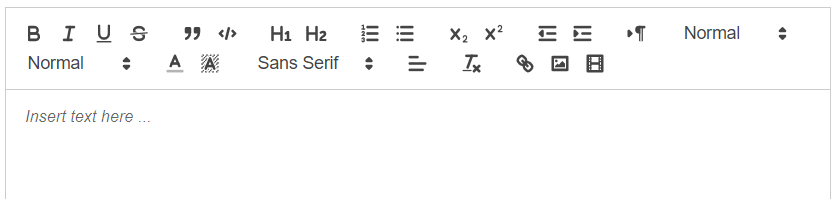
\includegraphics[
        width=0.9\textwidth, width=\linewidth, frame
        ]{images/quill.png}}
    \caption{Monaco code editor component}
    \label{fig:monaco}
\end{figure}


The second one is based on Monaco code editor, which powers a high productivity Visual Studio Code editor. This component was chosen because it  and has numerous tools to create a powerful development environment. The editor enables highlighting of the Java code, searching, suggestions, minimap, so the requirement of providing a close to conventional IDE was met.

\begin{figure}[h]
    \centerline{
        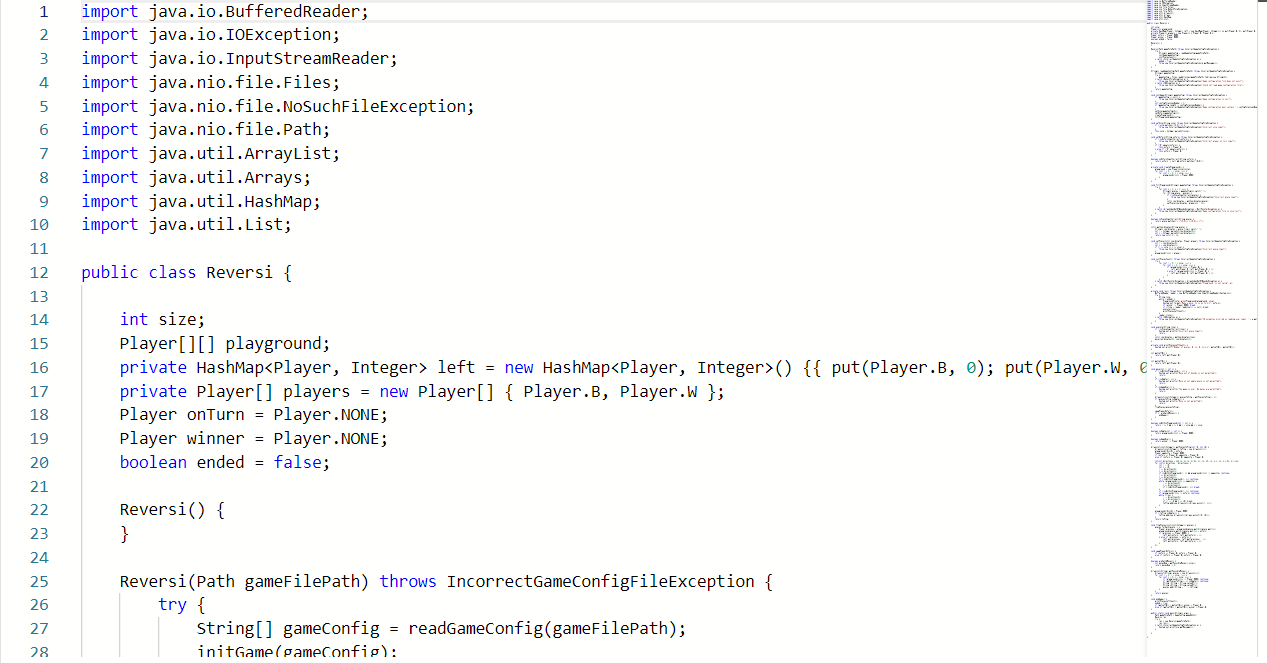
\includegraphics[
        width=0.9\textwidth, width=\linewidth, frame
        ]{images/monaco.png}}
    \caption{Quill text editor component}
    \label{fig:monaco}
\end{figure}

% dynamic form
Angular Form Group was used to create dynamic forms. They allow storing inputs from the user or generate multiple nested forms with the same structure. They were used to create and edit courses, lessons and exercises, and also to solve the latter. As a result, it is possible to change the form view as soon as different exercise type is selected. Also they are used to add, remove and rename files at the code editors on exercise creation.

Accuracy and completeness of the input is improved with the form validation, provided by the Form Group. The required fields change dynamically with the form itself.

% custom components
Most of the used components are custom. They are used to display pages or sections. Components are reusable, so some of them are used for different purposes, e.g. to create and edit a course, to manage a course and a lesson. Also they are used to display repetitive sections to avoid duplicates, e.g. show three same code editors with different content.


\subsection{Use cases}
The main page provides a list of the created courses and information on them. The user may choose one of the listed courses to enter it. Also the user may manage the courses, i.e. create, edit or delete them, with the use of the button. This and the rest of the pages contain ``Back`` button for easier navigation.

Each course page contains an information about it. There is an expansion panel below with lessons and exercises they include. Every lesson and exercise may managed as well. Management includes lesson editing, deleting, reordering and creation.

The pages, which contain the exercises, have the same core structure. There are two equal toolbars, one on the top and second on the bottom of the page. They contain the mentioned ``Back`` button, navigation within the lesson exercises, and there is a flag representing the progress on the solving current exercise. They change dynamically on the exercise change.

\begin{figure}[h]
    \centerline{
        
\includegraphics[
        width=0.9\textwidth, width=\linewidth, frame
        ]{images/toolbar.png}}
    \caption{Exercises toolbar}
    \label{fig:monaco}
\end{figure}


\section{Back-end}

\subsection{Virtual server}

\subsection{...}

\section{Database}

\subsection{...}

\section{Testing module}

\subsection{Virtual machine / Container}

\subsection{...}